\documentclass{article}

\begin{document}

\setlength{\parindent}{6ex}

\indent

In this section datasets and performance metrics will be explained. \par 
Datasets are used in training and testing of detectors. Datasets consist of some 
specific type of objects, in object detection case they are images, and the 
corresponding ground-truth information about the categories in images that 
detector performs to detect. So, the mainly used datasets are Pascal Visual Object 
Classes (VOC) \cite{pascalvoc} and Microsoft COCO: Common Objects in Context 
\cite{mscoco}. \par

Pascal VOC datasets are formed based on two challenges: classification and detection. From the 
beginning year of 2005 to 2012, Pascal VOC challenges are developed. Number of classes and images 
are increased through challenges. The last challenge of Pascal VOC is occured in 2012. Dataset of 
2012 consists of 20 categories in 11.530 images. \par

MS COCO aims to present a dataset in which common objects are in their natural 
contexts. The data are taken from complex everyday scenes. COCO consists of 91 
object categories in 328k images. A comparison between Pascal VOC and MS COCO 
of instances per category is shown in figure \ref{fig:cocovspascal1}. \par

Another dataset we used to test analyzed detectors is Multiple Object Tracking Benchmark 
(MOT) \cite{mot}. Although MOT is a dataset for tracking, in challenge MOT17Det, they provide a 
challenge for Pedestrian Detection. There are seven different video data provided for 
training set with their ground-truth labels. We used this data as test set. There are 
5316 frame to process with total of 112297 pedestrians annotated. 

\begin{figure}
    \centering
    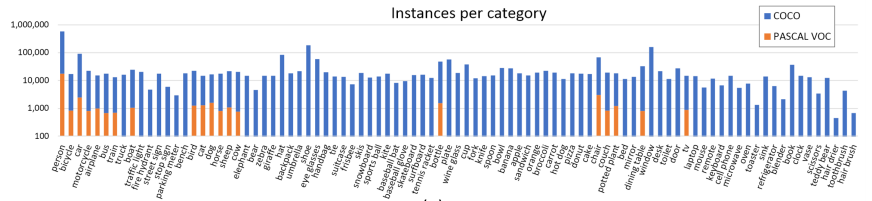
\includegraphics[width=\textwidth]{cocovspascal}
    \caption{Instances per category}
    \label{fig:cocovspascal1}
\end{figure}
\indent

Performance metrics are the way to measure the accuracy of detectors. In object 
detection, improving precision and recall yields to better test performance. The 
difference lies under the calculation of these metrics for object detection since 
correctly classifying the object in the image is not enough, detector also correctly 
localize the object in the image. So, to measure the correctness of each detection, 
a metric called Intersection over Union is used:

\begin{figure}
    \centering
    
\includegraphics[width=\textwidth]{iou}
    \caption{A visualization of IoU}
    \label{fig:iou1}
\end{figure}

\begin{table}[]
    \centering
    \begin{tabular}{|c|c|c|c|}
    \hline
    \multicolumn{2}{|c|}{\multirow{2}{*}{}}                                               & \multicolumn{2}{c|}{Ground-truth Value}                                         \\ \cline{3-4} 
    \multicolumn{2}{|c|}{}                                                                & Positive       & Negative                                                 \\ \hline
    \multirow{2}{*}{\begin{tabular}[c]{@{}c@{}}Predicted\\ Value\end{tabular}} & Positive & True Positive  & \begin{tabular}[c]{@{}c@{}}False\\ Positive\end{tabular} \\ \cline{2-4} 
                                                                               & Negative & False Negative & \begin{tabular}[c]{@{}c@{}}True\\ Negative\end{tabular}  \\ \hline
    \end{tabular}
    \caption{Table to understand concepts of classification of a prediction}
    \label{table:1}
\end{table}

\begin{itemize}
    \item Intersection over Union (IoU)
    IoU is the ratio between the intersection of predicted and ground-truth bounding box 
    divided by union of predicted and ground-truth bounding box. The figure \ref{fig:iou1} is a 
    visualization of IoU to help to have a better intuition.
    \item Correctness of Detection
    IoU is used as a threshold to identify a detection as positive or negative. The 
    most commonly used IoU threshold is 0.5 which means if IoU value of a detection is 
    bigger than 0.5, that detection is counted as True Positive; otherwise, False Positive.
    \item The following concepts are used by the metrics:
    \begin{itemize}
        \item True Positive (TP): A correct detection, IoU $\geq$ threshold. 
        \item False Positive (FP): A wrong detection, IoU $\leq$ threshold.
        \item False Negative (FN): A ground-truth not detected.
        \item True Negative (TN): Since there are many possible bounding boxes that 
        do not contain any object, counting corrected misdetection is not necessarily 
        needed.
        \item A better intuition can be obtained by looking into table \ref{table:1}.
    \end{itemize}
    \item These calculated concepts above are used to measure two main metrics: precision and 
    recall. Precision is the ratio of true positives to the sum of true positives and false 
    positives which provides the ratio of how accurate is your predictions. Recall is the ratio 
    of true positives to the sum of true positives and false negatives which indicates the ratio of 
    finding positives in all positives.
    \item The performance indicator for detectors is mean average precision. Average precision of a 
    category can be calculated by calculating the area under precision-recall curve. Then, the mean 
    average precision is calculated by calculating average precision for all categories and divide 
    this total AP by the number of categories. In Pascal VOC, AP is calculated by using interpolation. 
    11-point interpolated precision-recall curve is used. Corresponding precision values of 11 recall 
    points are summed up and this value is divided by 11. Another way is to calculate all area under 
    the precision-recall curve which is used in later year competetions of Pascal VOC. In MS COCO, 
    101-point interpolated AP calculation is used. In MOT17Det, 11-point interpolated AP is used.  
\end{itemize}
\end{document}